\newpage
\section{Metodologia Experimental}

Este experimento foi dividido em 2 circuitos.


\subsection{Circuito 1}
Para o circuito mostrado na figura \ref{f_cir1}:

\begin{itemize}
\item calcular o ganho na banda de passagem;
\item calcular a frequência de corte;
\item simular o circuito com o software Orcad;
\item gerar o gráfico da resposta em frequência do circuito;
\item determinar o ganho na banda de passagem simulado;
\item determinar a frequência de corte do circuito simulado;
\item determinar o tipo de resposta (Butterworth, Chebyshev, Bessel, etc.);
\item determinar a ordem do filtro e a atenuação em DB/década;
\item comparar os resultados teóricos com o simulado.
\end{itemize}

\begin{figure}[H]
\centering
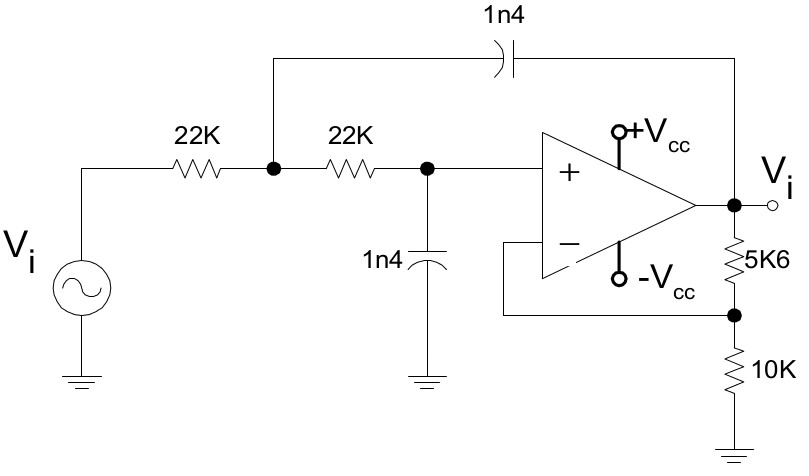
\includegraphics[scale=0.3]{Imagens/cir1.jpg}
\caption{Filtro ativo passa-baixas.}
\label{f_cir1}
\end{figure}



\subsection{Circuito 2}
Para o circuito mostrado na figura \ref{f_cir2}:

\begin{itemize}
\item calcular a frequência de corte para o primeiro estágio do filtro;
\item simular o primeiro estágio e comparar a resposta em frequência obtida com o resultado teórico;
\item calcular a frequência de corte para o segundo estágio do filtro;
\item simular o segundo estágio e comparar a resposta em frequência obtida com o resultado teórico;
\item simular o circuito em cascata com o inversor no software Orcad e obter a resposta em frequência;
\item determinar o ganho na banda de passagem simulado;
\item determinar a frequência de corte do circuito;
\item determinar o tipo de resposta (Butterworth, Chebyshev, Bessel, etc.);
\item determinar a ordem do filtro e a atenuação em DB/década;
\item comparar os resultados teóricos com o simulado.
\item inserir uma forma de onda quadrada de frequência fundamental igual a 90\% da frequência de corte encontrada e analisar a forma de onda na saída.
\end{itemize}

\begin{figure}[H]
\centering
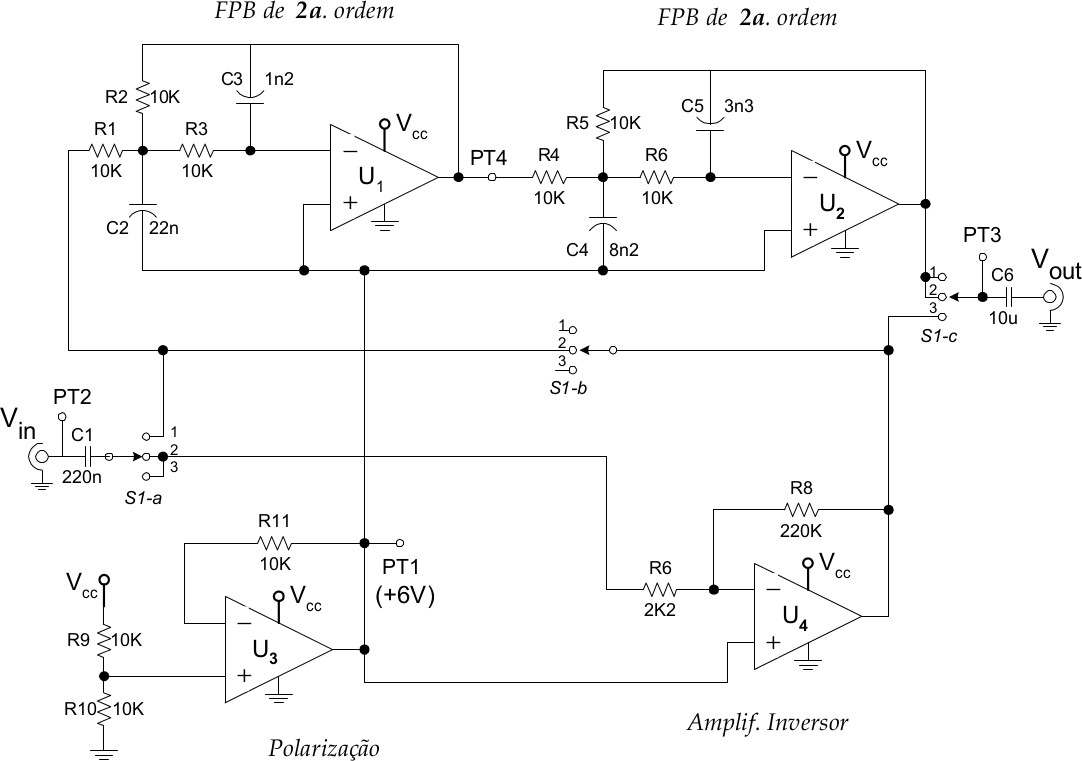
\includegraphics[scale=0.2]{Imagens/cir2.jpg}
\caption{Filtro ativo passa-baixas em cascata com circuito de polarização.}
\label{f_cir2}
\end{figure}